\section{Testing}
\subsection{Analisi statica}
Per l’analisi statica del codice Java é stato utilizzato il tool STAN4J, il seguente è il report generato a partire dal nostro codice.
\\
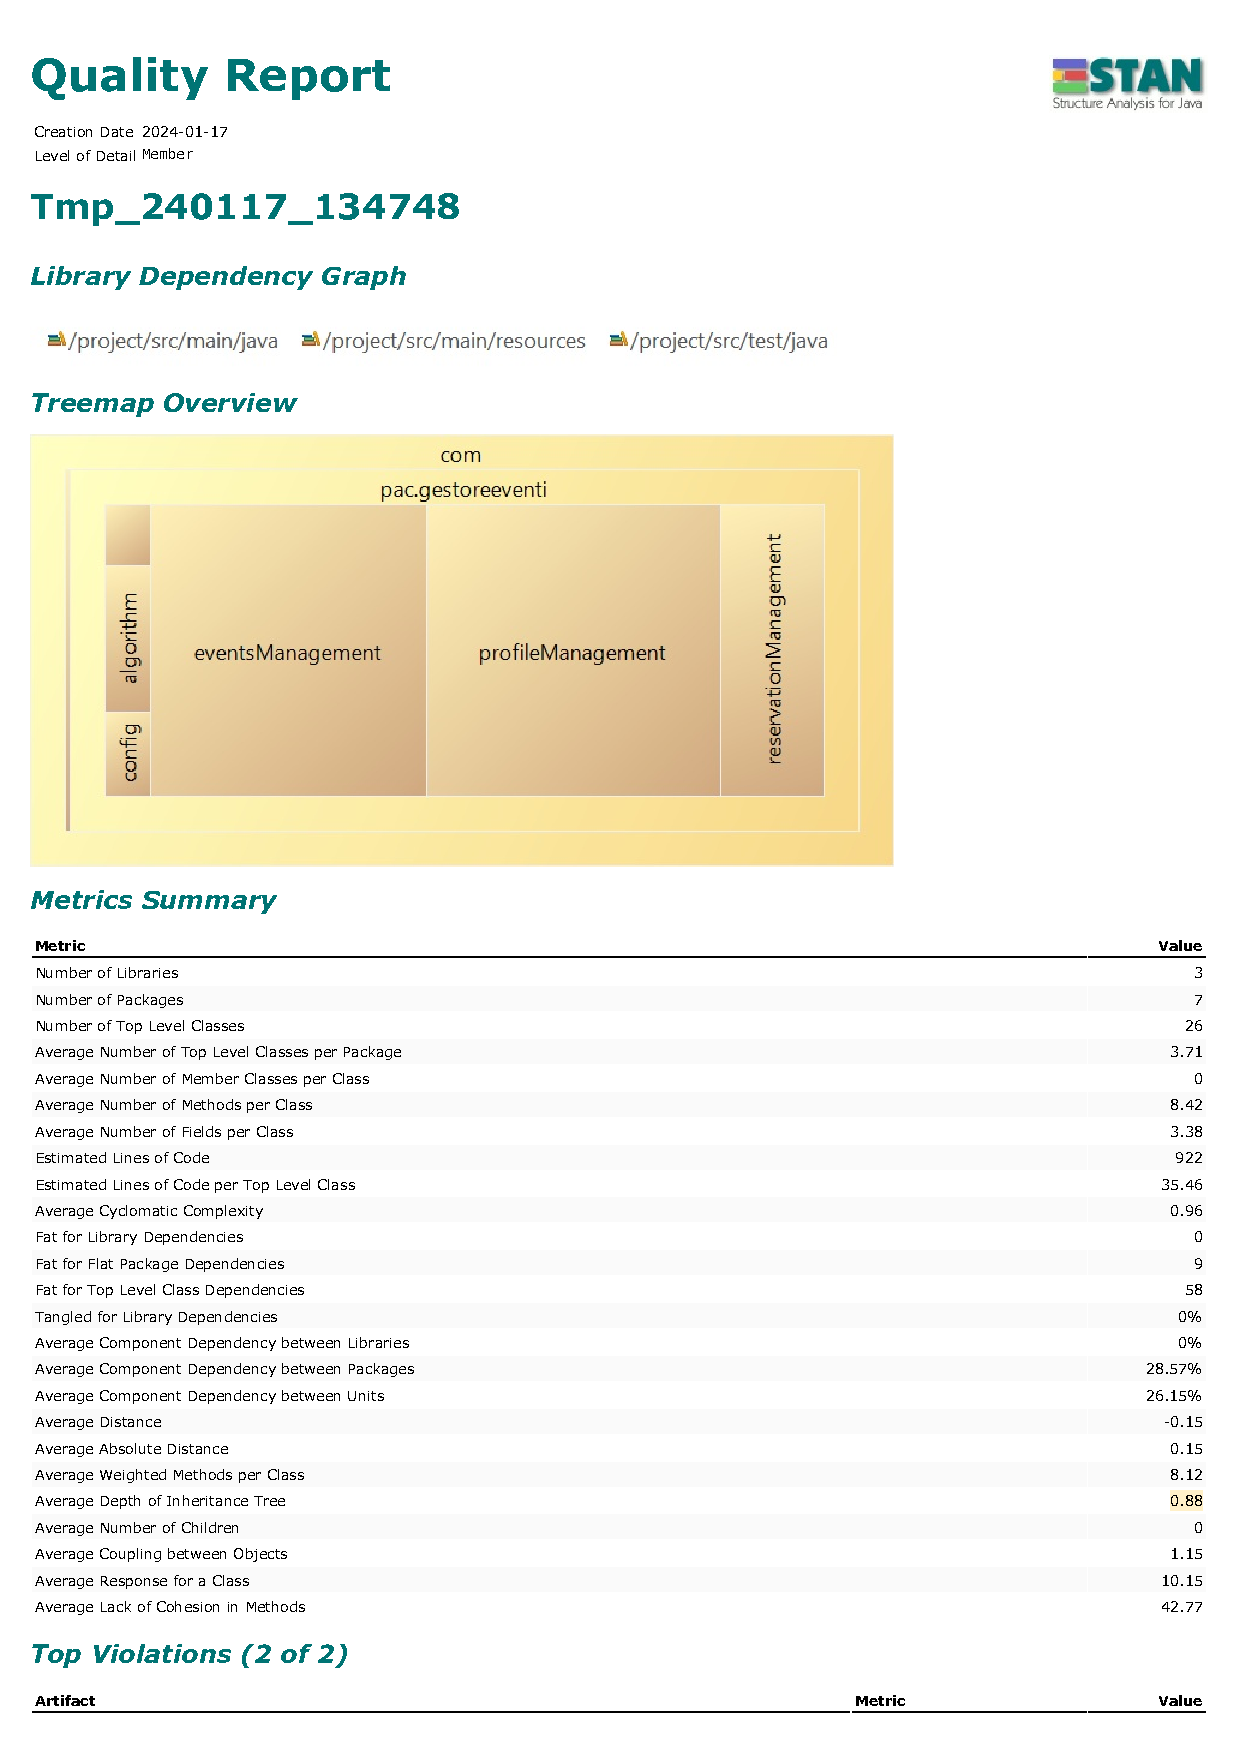
\includepdf[pages=-]{Documentazione/Iterazione 2/test/static analysis/static analysis.pdf}

\subsection{Analisi dinamica}
Nell’iterazione 2 sono state testate tutte le API REST implementate, utlizzando Postman .
In particolare sono state testate le seguenti funzionalita:

\begin{itemize}
	\item ProfileController:
	\begin{itemize}
		\item Visualizzazione di tutti i profili registrati nel sistema;
		\item Visualizzazione di un profilo specifico e verifica della correttezza dei dati ritornati;
		\item Eliminazione profilo;
		\item Inserimento di un nuovo profilo e verifica che i dati del profilo siano stati inseriti in modo corretto;
	\end{itemize}
	\item EventController:
	\begin{itemize}
		\item Visualizzazione di un evento e verifica che le informazioni ricevute siano corrette;
		\item Visualizzazione di tutti gli eventi inseriti nel sistema;
		\item Eliminazione di un evento;
		\item Inserimento di un evento;
	\end{itemize}
	\item ReservationController:
	\begin{itemize}
		\item Visualizzazione di una reservation e verifica che le informazioni ricevute siano corrette;
		\item Visualizzazione di tutte le reservation inserite nel sistema;
		\item Inserimento di una nuova reservation;
		\item Eliminazione di una reservation;
	\end{itemize}

\end{itemize}

\begin{figure}[h!]
\begin{center}
  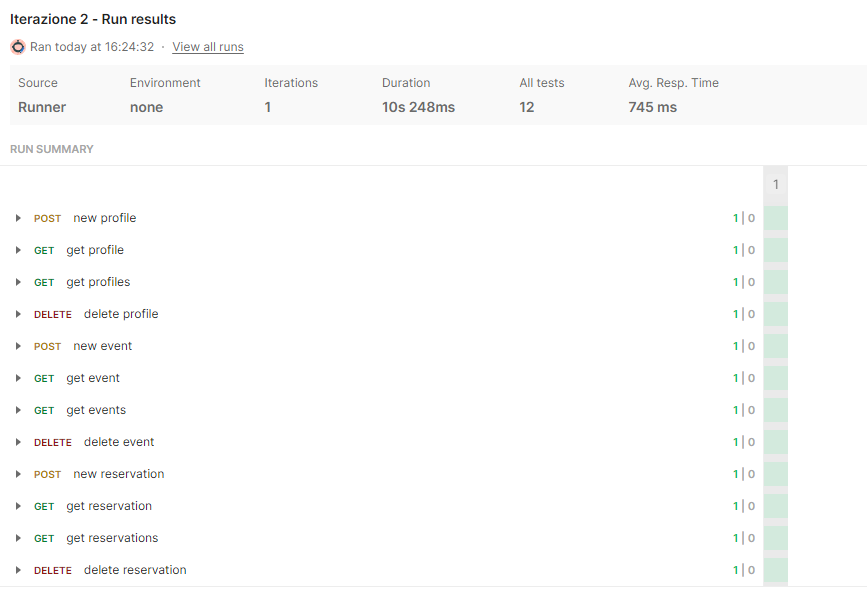
\includegraphics[width=14cm]{test/postman/collections.PNG}\\
  \caption{Test collection}
  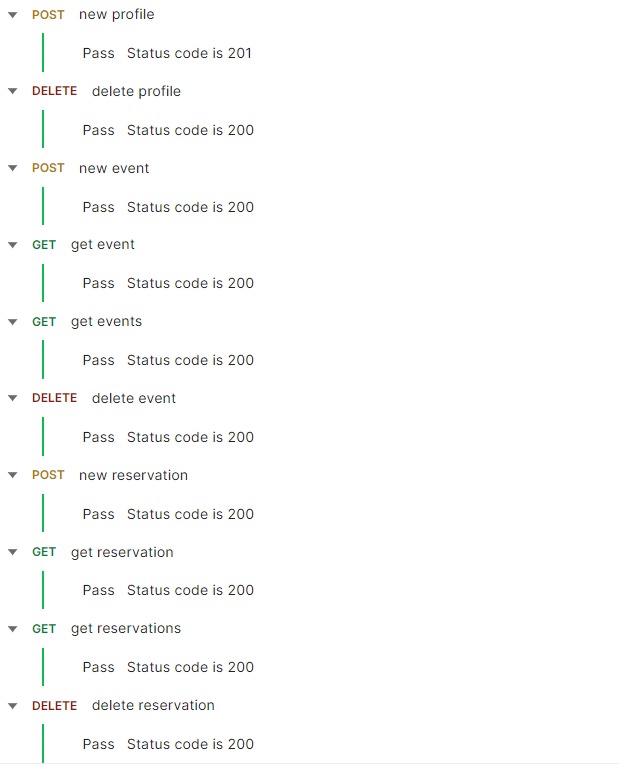
\includegraphics[width=30cm]{test/postman/collections sng.PNG}\\
\end{center}
\end{figure}
